\documentclass[]{beamer}
\usepackage{tikz,lstautogobble,listings}
\usetikzlibrary{arrows.meta}
\usetheme{Rochester}
\usepackage[T1]{fontenc}
\usepackage[utf8]{inputenc}
\lstset{
  language=caml,
  basicstyle=\ttfamily\tiny,
  breaklines=true,
  autogobble=true,
}


\title{TIPE 25/26 - Cycles et Boucles}
\author{GIL Dorian}
\subtitle{Méthode des tableaux : Optimisation et étude de la satisfiabilité de formule}
\date{}

\begin{document}

\begin{frame}
\titlepage
\end{frame}

\begin{frame}{Sommaire}
\begin{enumerate}
    \item Où on s'est quitté
    \item Ce que j'ai fait
    \item Objectifs futurs
\end{enumerate}
\end{frame}

\begin{frame}{Où on s'est quitté}
    On s'était quitté la dernière fois sur une discussion sur l'orientation du questionnement de mon TIPE.

    La remarque principale étant que je devais faire mon étude de la méthode des tableaux sur une forme particulière de formule que je devais poser moi même.

    J'ai donc décidé en lien avec les remarques que vous m'avez fait de bien re-orienter mon TIPE.
\end{frame}

\begin{frame}{Ce que j'ai fait - Définition}
    \begin{definition}[Forme Alternée]
        Soit $n\in\mathbb{N}^*$, et $(a_k)_{k\in [|1,n|]}$ des litteraux, on dit que $\varphi$ est de forme alternée ssi
        $$\varphi = a_1\land(a_2\lor(a_3\land(\dots(a_n))))$$
    \end{definition}
    \pause
    \begin{theorem}
        \begin{itemize}
            \item Si $\varphi$ une forme alternée: $$\lnot\varphi = \lnot a_1\lor(\lnot a_2\land(\lnot a_3 \lor(\dots(\lnot a_n))))$$
            \item Chaque arbre induit des formes alternées par la méthode des tableaux peut être écrit comme un arbre binaire tel qu'on nomme dans les nodes les hypothèses, l'écriture est en $\mathcal{O}(n)$
        \end{itemize}
    \end{theorem}
\end{frame}

\begin{frame}{Ce que j'ai fait - Algorithme}
    En utilisant la 2ème propriétée, on peut trouver un moyen d'écrire l'algorithme de la méthode des tableaux, en utilisant la forme spéciale de l'arbre induit (exemple si dessous pour $n=5$)
    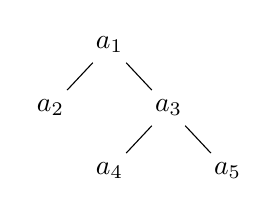
\begin{tikzpicture}[level distance=8mm]
        \node {$a_1$}
            child {node {$a_2$}}
            child {node {$a_3$}
            child {node {$a_4$}}
            child {node {$a_5$}}};
    \end{tikzpicture}
    $\varphi = a_1\land(a_2\lor(a_3\land(a_4\lor a_5)))$
    \pause

    On créé un dictionnaire. 
    On appelle litteraux droits les litteraux impairs et gauche les pairs:  
    \begin{enumerate}
        \item On analyse le litteral droit, si il y a contradiction, l'arbre est fermé, sinon on ajoute eventuellement dans le dictionnaire le litteral
        \item On analyse le litteral gauche, si il produit une contradiction, appel recursif plus profond dans l'arbre, sinon la formule est satisfiable
    \end{enumerate}
\end{frame}

\begin{frame}{Objectifs Futurs}
    Voici ce que j'aimerai faire pendant les grandes vacances
    \begin{enumerate}
        \item Trouver une formule plus difficile de la logique propositionelle à étudier.
        \item M'intéresser à la logique du premier ordre pour faire une ultime étude de la méthode des tableaux.
    \end{enumerate}
    Voir de possiblement de directement passer à une étude en logique du première ordre.
\end{frame}

\begin{frame}[fragile]{Code - Méthode des tableaux classique 1}
    \begin{center}
        \begin{tabular}{c}
            \begin{lstlisting}
                type formula =
                    | Atom of string
                    | Not of formula
                    | And of formula * formula
                    | Or of formula * formula

                let rec expand formula =
                    match formula with
                    | Not (Not f) -> [[f]]
                    | Not (And (f1, f2)) -> [[Not f1]; [Not f2]]
                    | Not (Or (f1, f2)) -> [[Not f1; Not f2]]
                    | And (f1, f2) -> [[f1; f2]]
                    | Or (f1, f2) -> [[f1]; [f2]]
                    | _ -> [];;

                let rec has_cycle branch =
                    List.exists (fun f -> List.mem (Not f) branch) branch;;
            \end{lstlisting}
        \end{tabular}
      \end{center}
\end{frame}

\begin{frame}[fragile]{Code - Méthode des tableaux classique 2}
    \begin{center}
        \begin{tabular}{c}
            \begin{lstlisting}
                let rec tableau branches =
                    match branches with
                    | [] -> false
                    | branch :: rest -> 

                    if has_cycle branch then
                        tableau rest
                    else
                        match branch with
                        | [] -> true
                        | f :: fs ->

                        let expansions = expand f in match expansions with
                        | [] -> tableau (fs :: rest)
                        | new_branches ->
                        
                        let expanded_branches = List.map (fun b -> b @ fs) new_branches in
                        tableau (expanded_branches @ rest);;

                    let is_satisfiable formula =
                    let initial_branch = [formula] in tableau [initial_branch];;
            \end{lstlisting}
        \end{tabular}
    \end{center}
\end{frame}

\begin{frame}[fragile]{Code - Alternée 1}
    \begin{center}
        \begin{tabular}{c}
            \begin{lstlisting}
                type formula =
                    | Atom of (string* bool)
                    | And of (string*bool) * formula
                    | Or of (string*bool) * formula

                type branch = 
                    | Empty
                    | Node of (formula option * formula * branch);;

                let extract (f:formula option) = match f with
                    | None ->  Atom("none", false)
                    | Some t -> t

                let rec print_formula (f:formula) = match f with
                    | Atom(s, b) -> if b then print_string s else print_string "Not ";print_string s;
                    | And ((f, b),g) -> if b then print_string f else print_string "Not ";print_string f;print_string " And ";print_formula g
                    | Or ((f,b),g) -> if b then print_string f else print_string "Not ";print_string f;print_string " Or ";print_formula g;;

                let rec print_branches (b:branch) =
                    print_string " [";
                    match b with
                        | Empty -> ()
                        | Node(a1, a2, b) -> print_formula@@extract a1;print_string ", ";print_formula a2;print_branches b;
                    print_string "]";; 
            \end{lstlisting}
        \end{tabular}
    \end{center}   
\end{frame}

\begin{frame}[fragile]{Code - Alternée 2}
    \begin{center}
        \begin{tabular}{c}
            \begin{lstlisting}
            let rec formula2branch (f:formula) : branch = match f with
                | And(a, Or(b, Atom(c))) -> Node(Some(Atom b), Atom a, Node(None, Atom(c), Empty))
                | And(a, Or(b, c)) ->  Node(Some(Atom b), Atom a, formula2branch c)
                | And(a, Atom(b)) -> Node(Some (Atom b), Atom a, Empty)
                | _ -> failwith "Pas alternee"
              
            let has_cycle (br:branch) : bool = 
                let rec aux (br:branch) (d:(string,bool) Hashtbl.t) : bool = match br with
                | Node(None, Atom (f, b), Empty) -> 
                  if Hashtbl.mem d f then 
                    Hashtbl.find d f = b
                  else
                    true
                | Node(Some(Atom(fg, bg)), Atom (fd, bd), Empty) -> 
                      if Hashtbl.mem d fd then
                        if Hashtbl.find d fd = bd then
                          not @@ Hashtbl.mem d fg && Hashtbl.find d fg <> bg
                        else 
                          false
                      else(
                        Hashtbl.add d fd bd;
                        not @@ Hashtbl.mem d fg && Hashtbl.find d fg <> bg)
                | Node(Some (Atom (fg, bg)), Atom (fd, bd), nb) ->
                  if Hashtbl.mem d fd then
                    if Hashtbl.find d fd <> bd then
            \end{lstlisting}
        \end{tabular}
    \end{center}   
\end{frame}

\begin{frame}[fragile]{Code - Alternée 3}
    \begin{center}
        \begin{tabular}{c}
            \begin{lstlisting}
                        false
                            else
                            if Hashtbl.mem d fg then
                                if Hashtbl.find d fg = bg then
                                true
                                else
                                aux nb d
                            else
                                true
                        else
                            (Hashtbl.add d fd bd;
                            if Hashtbl.mem d fg then
                            if Hashtbl.find d fg = bg then
                                true
                            else
                                aux nb d
                            else
                            true)
                        | _ -> failwith "Pas alternee"
                        in aux br (Hashtbl.create 100);;
          
                        let is_satisfiable (f:formula) : bool = let b = formula2branch f in has_cycle b;;
            \end{lstlisting}
        \end{tabular}
    \end{center}   
\end{frame}
\end{document}